\documentclass[12pt, class=report, crop=false]{standalone}
\usepackage{msc_thesis}

% !TeX spellcheck = en-GB
% !TEX bib = reference.bib
% chktex-file 21 # This command might not be intended.

\begin{document}

\chapter{Results}%
\label{chap:results}

In this chapter we present the main numerical results obtained with the EPOCH
Particle in Cell code. The simulations were performed using the computing cluster
at the Department of Computational Physics and Information
Technologies of the National Institute of Physics and Nuclear Engineering.
The servers used for simulations had an Intel\textsuperscript{®} Xeon\textsuperscript{®}
E5-2640 v4 CPU with a frequency of \SI{2.4}{\giga\hertz} (\SI{3.4}{\giga\hertz}
with Turbo Boost). Each server had 2 sockets with 10 cores per socket and
128GB RAM.\@ For simulations, we used MPI parallelisation on the cores of one
server, manually parallelising over parameters using multiple machines.
From benchmarks it was found that using Hyper-Threading (40 jobs per server)
was advantageous. The average simulation time was around 2--3 hours for solid
targets and 15--20 minutes for the gaseous targets.

In order to ensure the reproducibility of the results and to promote better
software practices the input decks required for the EPOCH simulations
as well as the \LaTeX\ code for this thesis are version controlled and
freely available online~\autocite{micluta-campeanu_sebastianmcmasterthesis_2019}.

There are multiple ways of accelerating particles via laser-plasma interactions.
One can classify these methods according to the target type, that is if the
target is solid or gaseous (under-dense). From the point of view of the physics, in the
case of a solid, the incoming electromagnetic wave does not propagate inside
the material, while in the case of a under-dense plasma, the laser propagates
through the media. From the point of view of the simulation, the difference is
given by the density of the simulated species. Thus the laser wakefield mechanism
is present only in the case where the laser propagates through the plasma.

\section{Solid target}

We begin with some simulations concerning solid targets following
\textcite{budriga_modelingultrahigh_2017}. For all the simulations we will consider
a plastic cone target interacting with an incoming laser pulse as shown in the
initial snapshot in \cref{fig:initial-plasma-laser}.

\begin{figure}[hb]
    \centering
    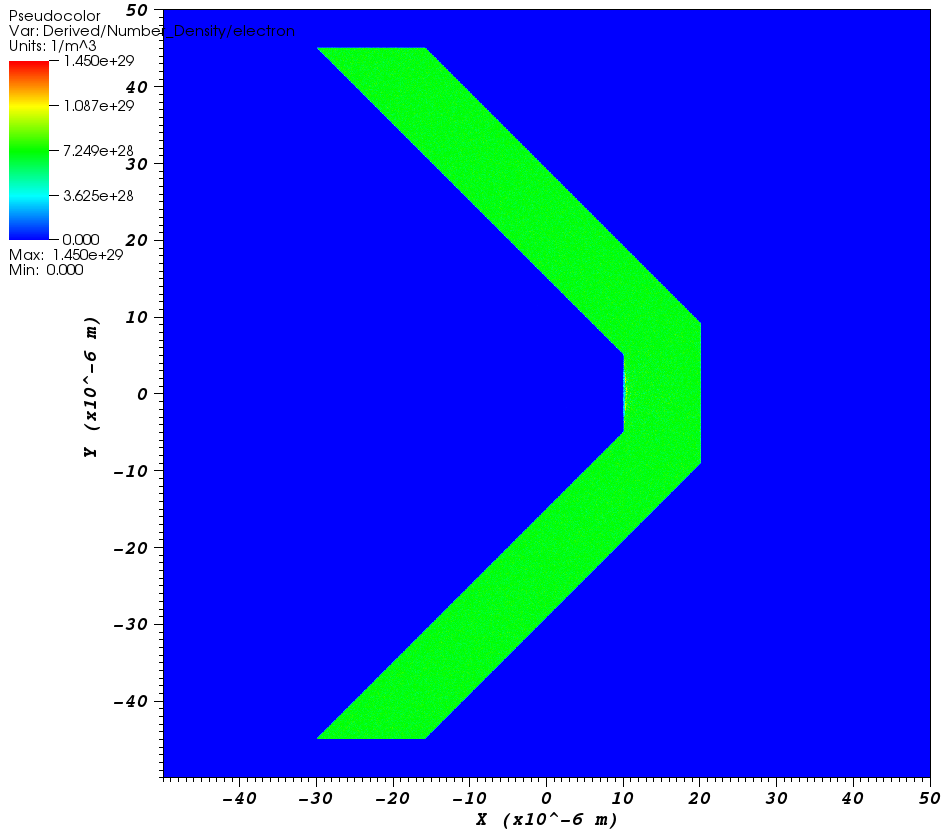
\includegraphics[width=0.65\textwidth]{i19-n-init-e}
    \caption{Initial configuration of the system}%
    \label{fig:initial-plasma-laser}
\end{figure}

The laser is modelled as a gaussian pulse with a focal spot FWHM
(full width at half maximum) of \SI{6}{\micro\metre}, yielding
a \(w_0=\SI{3}{\micro\metre}\) beam waist size. The laser has the
wavelength \(\lambda=\SI{800}{\nano\metre}\), the period
\(\tau_0=\SI{2.66}{\femto\second}\), the duration of
\(\tau=\SI{25}{\femto\second}\) and the maximum intensity between
\(I=\SI{e19}{\watt\per\centi\metre\squared}\) and
\(I=\SI{e22}{\watt\per\centi\metre\squared}\).
The laser is attached to the left boundary and is focused such
that the focal point is at the interior of the top of the cone.

The simulation domain is a square with a \SI{100}{\micro\metre}
side with 2750 cells in both \(O_x\) and \(O_y\) directions.
The left and right boundary conditions are open and the up and
down ones are periodic. The total simulation duration is \SI{1.5}{\pico\second}.

The plastic cone has an initial density of \(40n_c\), where \(n_c\)
is the critical density of the plasma. At the critical density, the
plasma frequency is equal to the laser frequency. The cone is has a
height of \SI{40}{\micro\metre}, wall thickness of \SI{10}{\micro\metre} and is made of plastic, that is modelled as
having in each cell 3 protons, 21 electrons and 3 ions with charge
6 and mass 21889 (expressed as function of the electron mass and elementary charge).

% \begin{figure}[h]
%   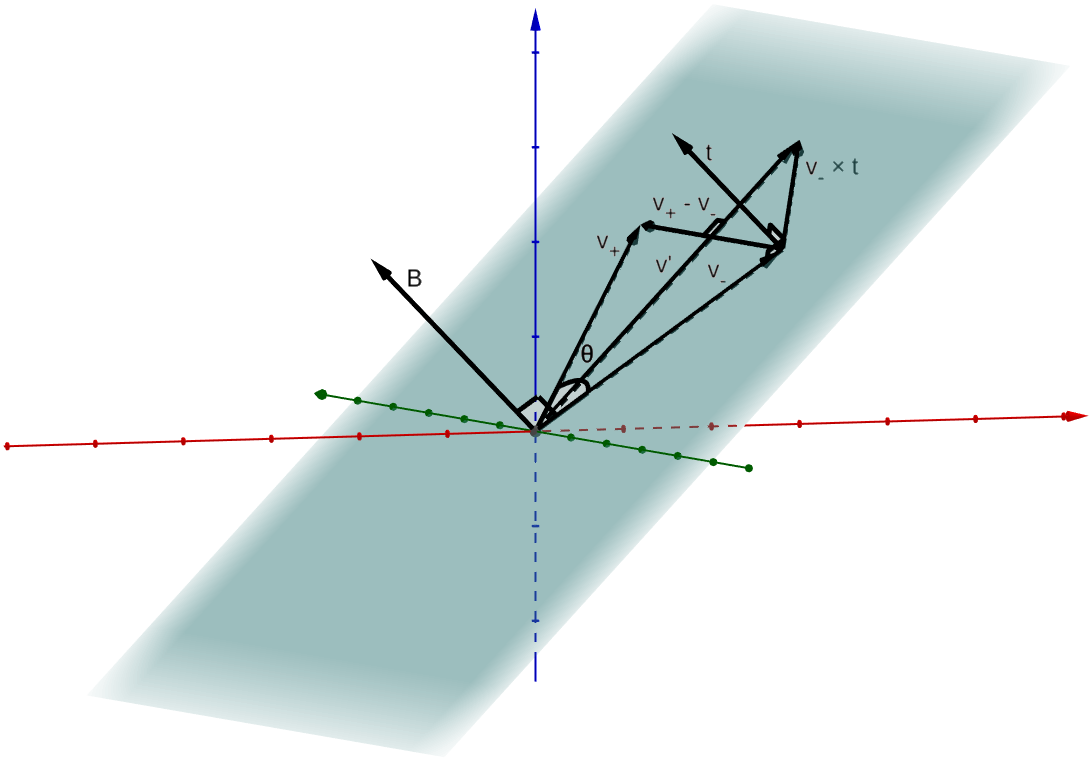
\includegraphics[width=\textwidth]{Boris-rotation-3D}
%   \caption{Boris rotation construction in 3D}%
%   \label{fig:Boris-rotation-3D}%
% \end{figure}


\section{Gaseous target}

We will now continue our study with gaseous targets. In this case
we will investigate how does the intensity of the laser pulse
contributes to the laser wakefield acceleration mechanism.
For this case, we are interested in the propagation of the laser
in the plasma and thus we will need a different target geometry.
We can consider that the plasma fills the entire space and since
the interesting physics only takes place in a relatively small
region, we can only observe and simulate only that part using a moving window.

Our numerical experiments with gaseous targets were limited with
respect to the power of the incoming laser pulse to around
1e18 PW. For higher powers of the incoming laser pulse, we need
spatial integration domains considerably higher which for powers
higher than 1e19 PW raise the physics becomes more complex and
requires more computational resources. For instance, for an
incoming laser pulse of 2e18 PW, we see an effective depletion
of the simulation domain which is unphysical and is due to the
absorbtive boundary conditions. In a nutshell, the laser pulse is
too strong for a domain of this size and particles are effectively
pushed out of the system through the absorbative boundaries.

(insert fig)

\end{document}
